%% 
%% Copyright 2007-2020 Elsevier Ltd
%% 
%% This file is part of the 'Elsarticle Bundle'.
%% ---------------------------------------------
%% 
%% It may be distributed under the conditions of the LaTeX Project Public
%% License, either version 1.2 of this license or (at your option) any
%% later version.  The latest version of this license is in
%%    http://www.latex-project.org/lppl.txt
%% and version 1.2 or later is part of all distributions of LaTeX
%% version 1999/12/01 or later.
%% 
%% The list of all files belonging to the 'Elsarticle Bundle' is
%% given in the file `manifest.txt'.
%% 

%% Template article for Elsevier's document class `elsarticle'
%% with numbered style bibliographic references
%% SP 2008/03/01
%%
%% 
%%
%% $Id: elsarticle-template-num.tex 190 2020-11-23 11:12:32Z rishi $
%%
%%
\documentclass[preprint,3p]{elsarticle}

%% Use the option review to obtain double line spacing
%% \documentclass[authoryear,preprint,review,12pt]{elsarticle}

%% Use the options 1p,twocolumn; 3p; 3p,twocolumn; 5p; or 5p,twocolumn
%% for a journal layout:
%% \documentclass[final,1p,times]{elsarticle}
%% \documentclass[final,1p,times,twocolumn]{elsarticle}
%% \documentclass[final,3p,times]{elsarticle}
%% \documentclass[final,3p,times,twocolumn]{elsarticle}
%% \documentclass[final,5p,times]{elsarticle}
%% \documentclass[final,5p,times,twocolumn]{elsarticle}

%% For including figures, graphicx.sty has been loaded in
%% elsarticle.cls. If you prefer to use the old commands
%% please give \usepackage{epsfig}

%% The amssymb package provides various useful mathematical symbols
\usepackage{amssymb, amsthm}
\usepackage{amsmath}
%% The amsthm package provides extended theorem environment
\usepackage{subcaption}
\usepackage[T1]{fontenc}
\usepackage{babel}
\usepackage{wrapfig}
\usepackage{geometry}
\usepackage{fancyref}
%% The lineno packages adds line numbers. Start line numbering with
%% \begin{linenumbers}, end it with \end{linenumbers}. Or switch it on
%% for the whole article with \linenumbers.
\usepackage{lineno}

\journal{Journal of Quantitative Spectroscopy $\&$ Radiative Transfer}

\begin{document}

\begin{frontmatter}

%% Title, authors and addresses

%% use the tnoteref command within \title for footnotes;
%% use the tnotetext command for theassociated footnote;
%% use the fnref command within \author or \address for footnotes;
%% use the fntext command for theassociated footnote;
%% use the corref command within \author for corresponding author footnotes;
%% use the cortext command for theassociated footnote;
%% use the ead command for the email address,
%% and the form \ead[url] for the home page:
%% \title{Title\tnoteref{label1}}
%% \tnotetext[label1]{}
%% \author{Name\corref{cor1}\fnref{label2}}
%% \ead{email address}
%% \ead[url]{home page}
%% \fntext[label2]{}
%% \cortext[cor1]{}
%% \affiliation{organization={},
%%             addressline={},
%%             city={},
%%             postcode={},
%%             state={},
%%             country={}}
%% \fntext[label3]{}

\title{Investigating the Applications and Limits of Single asymmetric Particle Light Scattering using Limited Detection Schemes}

%% use optional labels to link authors explicitly to addresses:
%% \author[label1,label2]{}
%% \affiliation[label1]{organization={},
%%             addressline={},
%%             city={},
%%             postcode={},
%%             state={},
%%             country={}}
%%Saffran
%% \affiliation[label2]{organization={},
%%             addressline={},
%%             city={},
%%             postcode={},
%%             state={},
%%             country={}}

\author[aff1]{Dan Maciver\corref{cor1}} %
\ead{Daniel.Maciver.2016@uni.strath.ac.uk}

\author[aff1]{Praveen Parthasarathi}

\author[aff1]{Mark Haw}

\author[aff1]{Leo Lue}

\author[aff1]{Jan Sefcik}

\cortext[cor1]{Corresponding author}
\affiliation[aff1]{organization={Department of Chemical Engineering,
			University of Strathclyde},
            addressline={75 Montrose Street}, 
            city={Glasgow},
            postcode={G1 1XL}, 
            country={Scotland}}


\begin{abstract}
While optical trapping is a well understood method for force transduction and detection,characterisation of trapped entities poses a two-fold challenge - one experimental concerning the arrangement of light detectors and the other, theoretical involving solving of the inverse light scattering problem. Combining static light scattering techniques with optical trapping poses significant engineering challenges due to the space constraints in a conventional optical trapping setup. We propose here a plausible scenario of detecting scattered light from an optically trapped asymmetric microstructure using a novel, multi-angle, optical-fibre based detection scheme and demonstrate how a Bayesian inference based analysis of the data simulated to mimic light scattering detection signals in such scenarios maybe used for solving the inverse light scattering problem and help characterise trapped entities. To this end, we discuss the application of our method to infer the instantaneous orientations of an asymmetric microsphere dimer being trapped. We argue that this method can be extended for determining any characteristics of the trapped microstructure that influence the light scattering pattern.
\end{abstract}
%%Research highlights
\begin{highlights}
\item Asymmetric dimers of undergo a full inversion in the presence of an potential well
\item Orientation can be classified by applying Bayesian Statistics to light intensity readings
\item Bayesian model shows increased accuracy when processing noisy signal measurements. 
\item Multiple estimations can be  used to cancels out artefacts of noise. 
\end{highlights}

\begin{keyword}
	Optical Trapping \sep Light Scattering \sep Measurements \sep Bayesian Statistics \sep Theoretical 
\end{keyword}

\end{frontmatter}

\linenumbers

%% main text
\section{Introduction}
\label{sec:Intro}

\indent Since their invention in the late 1980's, Optical Tweezers have found application in experiments ranging from single molecule biophysics \cite{Bustamante2021Biophysics} to those that test the fundamental assumptions of Quantum Mechanics  \cite{yin2013large} thanks mainly to the ability of the tweezer to transduce and detect forces in the order of a few piconewton. Recent applications of the Optical Tweezers in metrological measurements \cite{arita2020coherent} and colloidal aggregation \cite{burns1990optical} demand the tweezer to also be able to characterise  the trapped entity. To this end, chemical characterisation of the trapped entities has been achieved using spectroscopic techniques such as Raman Scattering \cite{gupta2014raman} and dynamical characterisation has been achieved mainly by following the centre-of-mass Brownian motion of the trapped entity using a Quadrant Photo Detector \cite{friedrich2012tuning}. 
\begin{wrapfigure}[12]{r}{0.3\textwidth}
	\centering
	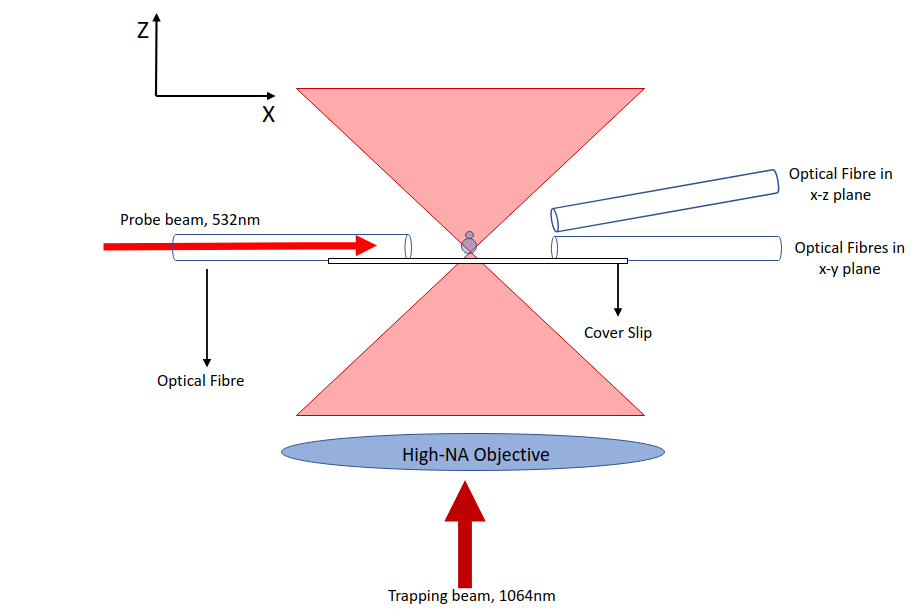
\includegraphics[width=0.3\textwidth]{fig1a}
	\caption{Experimental set up}
	\label{fig:1}
	\vspace{-100pt}
\end{wrapfigure}
While this technique has allowed for detection of linear motion of trapped entities  with sub-nanometre precision \cite{friedrich2012tuning} and  rotation \cite{yifat2021facile} of the centre-of-mass, there is a paucity of literature on measuring the orientation of trapped non-spherical particles till the recent attempt in \cite{raudsepp2022estimating} where imaging was employed to study the orientation of trapped dimers and a resolution of () was achieved.   
Possibility of integrating light scattering with optical trapping was demonstrated by Saffran and co-workers in \cite{Bar-Ziv_1998} where a single-mode optical fibre was aligned to detect the scattered light from a trapped bead and it's Brownian motion was studied. While this allowed for studying the dynamics, any information with regards structure of the trapped bead was precluded as the measurement was a single-angle scattering measurement.
\newpage
In this work, we propose a novel Bayesian Inference based technique to interpret light scattering data detected in a scheme that expands on the technique in \cite{Bar-Ziv_1998} to detect scattered light simultaneously at 3 angles as shown in Figure~\ref{fig:1}.  

\section{Theory}
\label{sec:Theory}

Consider a dimer with unequal sphere diameters $a_1, a_2$ in an optical trap in some orientation $\hat{s}$. Due to the Brownian motion from the surrounding fluid the dimer's orientation changes with time. Assuming we cannot accurately determine the dimer's orientation from imaging alone we instead rely on it's light scattering. Rather than directly calculate the orientation vector we instead discretise the orientation space into 30 reference orientations. See \ref{Appendix 1} for the exact numerical values of reference orientations. The following records how we apply a Bayesian model to determine the estimate the closest reference orientation based on an instantaneous light scattering measurement. 

We use a Fortran package specialised for calculating non spherical t-matrices (MSTM) \cite{Mishchenko1996MSTM} to determine the light scattering intensity of our dimer in each reference orientation. The raw signal intensities for at 3 different angles ($\theta_1, \ \theta_2, \ \& \ \theta_3$) are calculated and then scaled down so that the signal response $y_k$ is normalised for each angle $k$:

\begin{align}
	y_k(\hat{n}) = 
	 \frac{\left[I(\hat{n}, \ \theta_k)- \langle I(\hat{n}, \ \theta_k) \rangle \right]} 
	{\langle I^2(\hat{n},\ \theta_k) \rangle -\langle I(\hat{n}, \ \theta_k)\rangle^2}
\end{align}

See \ref{Appendix 1} for a breakdown of the raw intensities and scaled signal responses. To classify the particle's orientation we compare the produced light scattering signal to a collection of reference orientations that are evenly spaced around the orientation space. We assume that the for each detection fibre the intensities can be distributed on a Gaussian curve centred at $y_k$, the normalised intensity at detection fibre k. Based on the light scattering from the dimer we can assign a probability that the produced light scattering pattern belongs to the reference orientation $\hat{n}$

\begin{align}
	p(y(\hat{s})\parallel\hat{n}) =& \Pi^3_{k=1}
	(2\pi\sigma^2)^{-1/2} \nonumber \\     &e^{-(y(\hat{n})_k-y(\hat{s})_k)^2/2\sigma^2}
\end{align}

Where $\sigma$ is the minimum distance between our reference orientations signals ($y_1, \ y_2, \ \& \ y_3$), . We can view this result as a conditional probability, if the orientation is determined ($\hat{n}$) then what is the probability that expected scattering signal matches our dimer's scattering signal. We instead want to know the inverse conditional, that with a given signal y the dimer was in orientation $\hat{n}$. We can calculate this using Bayes' theory:

\begin{align}
	p(\hat{n}\parallel y(\hat{s}))&= \frac{p(y(\hat{s})\parallel\hat{n})p(\hat{n})}{p(y)}
\end{align}

Where $p(\hat{n})$ and $p(y)$ are our estimations of the priori distributions of particle orientations and scattering signals respectively. The former can be estimated by some Boltzmann distribution based on the spacing between reference orientations. The latter priori $p(y)$ is the probability of our dimer producing the signal $y$ and is given as. 

\begin{align}
	p(y) = \int p(y(\hat{s})\parallel \hat{n}) p(\hat{n}) d\hat{n}
\end{align}

The inclusion of $p(y)$ normalises our probability distribution. In order to test the accuracy of our model we first test it using an idealised simulation of the target dimer. 

\subsection{Brownian Simulation}
\label{sec:2.1}
We use the Brownian OT package by Jerome Fung \cite{Vigilante2020Brownian_OT} to simulate how our target dimer moves while subject to an optical trap. The package is unique in that it combines MSTM \cite{Mishchenko1996MSTM} and 'Optical Tweezer Toolbox' (\textit{ott}) to simulate the motion of arbitrary shaped particles. 

For any trapped particle their are two major sources of motion, Brownian motion and optical forces. The Brownian displacement ($\Delta q^{\textbf{B}}$) is approximated by generating a set of normally-distributed numbers whose covariance is given by the dimer's diffusion tensor $\textbf{D}$. The diffusion tensor is computed based on Farsund's work \cite{Farsund1996}. 

\begin{align}
	\langle \Delta q_i^{\textbf{B}} \Delta q_j^{\textbf{B}}\rangle &= 2D_{ij} \Delta t 
\end{align}

For computing the optical force Brownian OT uses the T-Matrix method to calculate the scattering coefficients of the outgoing scattered wave. The T-matirx describes the scattering process by relating the scattering wave to the incident wave in an elegant equation.

\begin{align}
	\begin{pmatrix}
		p_{mn} \\
		q_{mn}
	\end{pmatrix}
	= \textbf{T}
	\begin{pmatrix}
		a_{mn} \\
		b_{mn}
	\end{pmatrix}
\end{align}

MSTM computes the T-matrix of the dimer, and then passes the T-matrix to \textit{ott} to compute the optical forces. The benefit of this approach is that MSTM can accurately compute the T-matrix for the dimer once and then \textit{ott} can calculate the optical force after each time step. The dimer displacement is the sum of both the optical and Brownian contributions. Brownian OT returns the displacement as a trajectory file; with the [x,y,z] position being relative to the trap focus, and the orientation being returned as a quaternion. 

For our model we simulate the motion of silica dimer trapped in a 5mW Gaussian beam; the dimer is comprised of two spheres with radii $1\\mu m, \ \& 0.5 \ \mu m$ respectively.  

\subsection{Testing our Model}
\label{sec:2.2}

Since MSTM has computed the T-matrix for our dimer, we can reuse it to calculate. We then apply \eqref{3} - covered in Section~\ref{sec:2.1} - to estimate the dimer orientation based on its scattering pattern. The priori estimate $p(\hat{n})$ is defined as a Boltzmann's distribution based on the normalised dot product of our previous estimation $\hat{n}_{t-\Delta t}$ and each reference orientation $\hat{n}_t$:

\begin{align}
	r_j(t, \hat{n})= \frac{1}{2}((\hat{n}_{t} \cdot \hat{n}_{t-\Delta t})-1) \\
	p(\hat{n})= \frac{e^{\beta (r_j(t,\hat{n})-1)}}
	{\Sigma_{i=1}^{30}e^{\beta(r_i(t, \hat{n})-1)}}
\end{align}

Where $\beta$ is a weighting factor that controls the significance of our priori estimate. Since we are testing with a simulation we already know the exact orientation of the dimer, we want to know how often our model can determine the closest reference orientation $\hat{n}$ to the true orientation $\hat{s}$, and how precise our prediction is. For a perfect model our probability distribution should equal 1 at the correct result and zero elsewhere. In reality our model will be some probability distribution that has some probability of any orientation being correct. To evaluate our model's accuracy and confidence we calculate the Kullback-Leibler divergence of the two probability distributions. 

\begin{align}
	K_{l, \#}(p_{guess} \parallel p_{ideal}) &= 
	p_{ideal} \nonumber \\ 
	&\ln \left[\frac{p_{ideal}}{p(\hat{n}\parallel y_k(\hat{s}))}
	\right]
\end{align}

Where the divergence goes to zero if $p_{ideal}=0$, for a single estimation this gives us an idea of how confident our model is in it's estimation. We sum the divergence of each measurement across the entire simulation to get an idea of how well the model performs across the entire simulation. To measure how much our result had improved we compare it to a worse case scenario, where every $\hat{n}$ is given uniform probability, and evaluate the improvement factor $F(K_l)$

\begin{align}
	K_{l, \ total} &= \sum\limits_{\# =1}^{timesteps} K_{l,\#} \\
	K_{l, \ worst} &= -\sum\limits_{\#=1}^{timesteps} \ln \left[\frac{1}{1/30} \right] \\
	F(K_l) &= \frac{K_{l,\ worst}}{K_{l, \ total}}
\end{align}

The worst case scenario can be akin to randomly choosing a reference orientation at each time step. Because our model is dependent on several parameters at once we need to a more sophisticated method for finding the optimum choice of parameters.  

\subparagraph{Optimization of parameters}
\label{2.3}
The efficacy of our estimation is a function of our detection angles, signal error, and weighting of $p(\hat{n})$. Evaluating every possible configuration manually is inefficient, therefore we utilised Ultra nest to apply a Monte Carlo simulation to our model. Ultra-nest is a sophisticated python package for fitting models with complex parameter interactions \cite{Buchner2016Ultranest}. Ultra-nest implements a variation of Monte Carlo integration, nested-sampling, where the likelihood contour is used to update a group of live points chosen from the prior estimation ($0^{\circ} \leq \theta_k \leq 180^{\circ}, \ 0 \leq \epsilon \leq 1, \ 0 \leq \beta \leq 5$).

We used the Ultra-nest software to create a set of live points of different choices of $\theta_1, \ \theta_2, \ \& \ \theta_3$, with each point being evaluated by its improvement factor ($F(K_l)$) produced. After evaluating every live point, the worst results are removed and new live points are created based on the information provided by the previous live points. This results in a convergence on parameter choices that result in an average divergence result of almost 0. A common issue with complex parameter spaces, such as ours, is the issue of degeneracies (where two or more parameters have identical parameter spaces), to combat this we implemented a random step sampler that selects a new live point some 'n' steps away in the parameter space.
 
\section{Results}
\label{3}
\subsection{Asymmetric dimer dynamics}
\label{3.1}
The Brownian OT software was used to simulate the motion of a trapped dimer ($a_1=1\mu m, a_2=0.5\mu m$) over the first 10 seconds of entering the optical trap. The initial orientation was assumed as strictly vertical (in line with the beam propagation direction). The dimer's position orientation was recorded every $10 \mu s$ for using as a test dataset for our model. 

\begin{figure}[t]
	\centering
	\begin{subfigure}{0.45\textwidth}
		\subcaption{}
		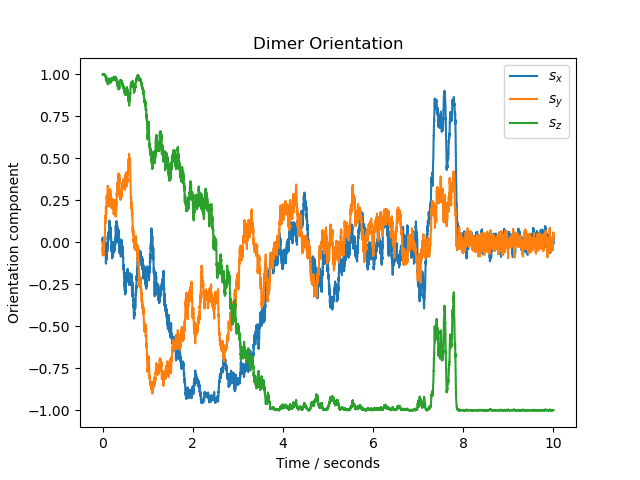
\includegraphics[width =\textwidth]{./Images/traj.png}
	\end{subfigure}
	\begin{subfigure}{0.45\textwidth}
		\subcaption{}
		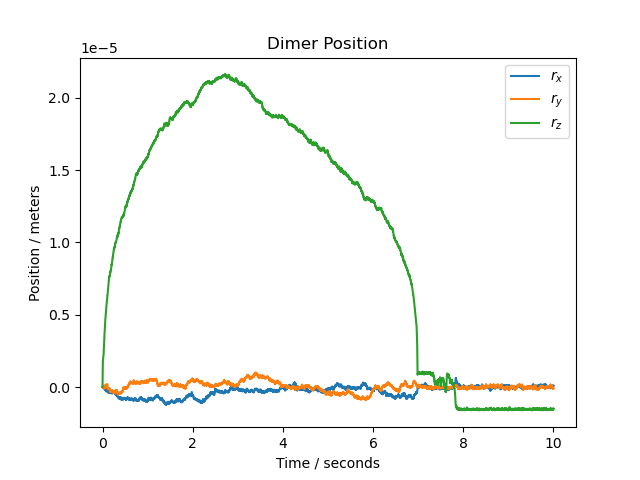
\includegraphics[width=\textwidth]{./Images/pos.png}
	\end{subfigure}
	\caption{Simulation results of: a) the dimers orientation vector with time, b) the dimer's [x,y,z] position with time.}
\end{figure}

As can be seen from \figurename{ 2}, the dimer undergoes a full $180^{\circ}$ rotation upon entering the trap. Typically horizontal alignment of a dimer is unstable and will result in the particle rotating to align along its vertical axis. It is interesting to note that the dimer is furthest from the trap centre as it goes into a horizontal orientation before drawing closer again as it inverts completely. Further simulations of differently sized dimers showed similar results, but only when $a_1 \geq 2a_2$. Dimers with more symmetrical size ratios immediately aligned into a fixed vertical position. 
In Vigilante's work with dimers \cite{Vigilante2020Brownian_OT} simulations of trapped symmetrical dimers was investigated; their findings showed that the optical torque on the dimer goes to zero while aligned vertically and is at its maximum in a horizontal alignment. Therefore, the inversion of an asymmetric dimer suggests that if the size difference is significant the optical torque goes is minimal for a dimer in both horizontal and vertical orientations. Once we have our experimental set up complete we can confirm this by trapping an asymmetric dimer and monitoring its orientation. The data from \figurename{ 2a} was used to test the efficacy of our predictive model. To visualise how well our model tracks the dimer's orientation we plot the radial distance between our model's prediction and the true orientation, and between the best possible orientation and the true orientation. For a perfect estimation these two plots should overlap, while  we cannot achieve an exact estimation there are several parameters that will effect our model's efficacy. 

\newpage
\subsection{Predictive efficacy of model}
\label{sec:3.2}
When we choose our three detction angles we are also inherently setting the lower limit for our signal error based on the minimum spacing between our $y_k$ values. If then signal error is smaller than this minimum distance then every refernce orientation will have the same probability $p(\hat{n} \parallel y_k)$ resulting in our model performing worse than just assigning reference orientations at random. We can reduce this minimum distance by creating more reference orientations thus increasing the accuracy of our predictive model. However if our signal error is to large then we are limited in how many refernece orienations we can use; futhermore, if the signal error is to large then our prediction can be. 

\begin{figure}[b]
	\begin{subfigure}{0.33\textwidth}
		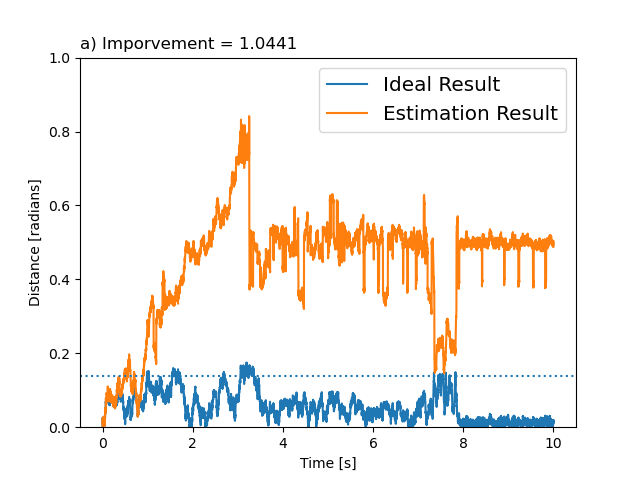
\includegraphics[width=\textwidth]{./Images/154590_Beta=1.png}
	\end{subfigure}
	\begin{subfigure}{0.33\textwidth}
		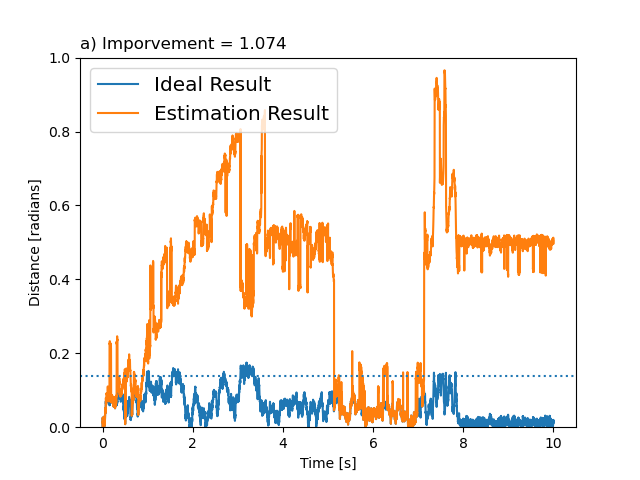
\includegraphics[width=\textwidth]{./Images/154590_Beta=05.png}
	\end{subfigure}
	\begin{subfigure}{0.33\textwidth}
		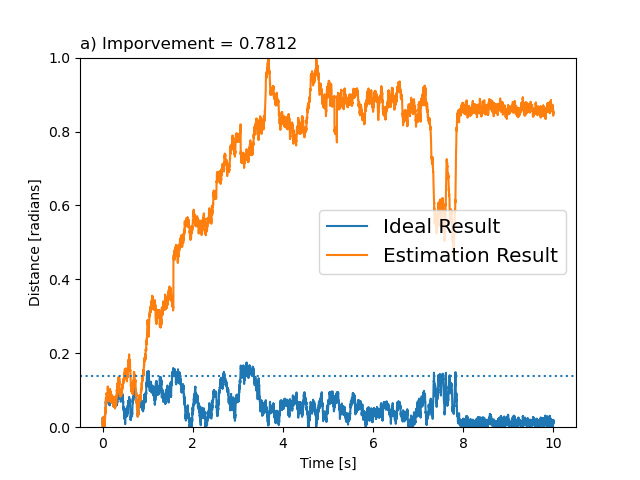
\includegraphics[width=\textwidth]{./Images/154590_Beta=15.png}
	\end{subfigure}
\end{figure}
 

\newpage
\subsection{Ultranest Results}
\label{3.3}
We wanted to see if our choice of angles plays a significant role in our model's efficacy. We employed ultranest to analyse the parameter space for our three angles by sampling across the priori of $10^{\circ} \ \& \ 180^{\circ}$. We kept both $\beta$ and $\sigma$ constant during this so we could as these are parameters that can be changed more freely. 

\begin{figure}[h]
	\centering
	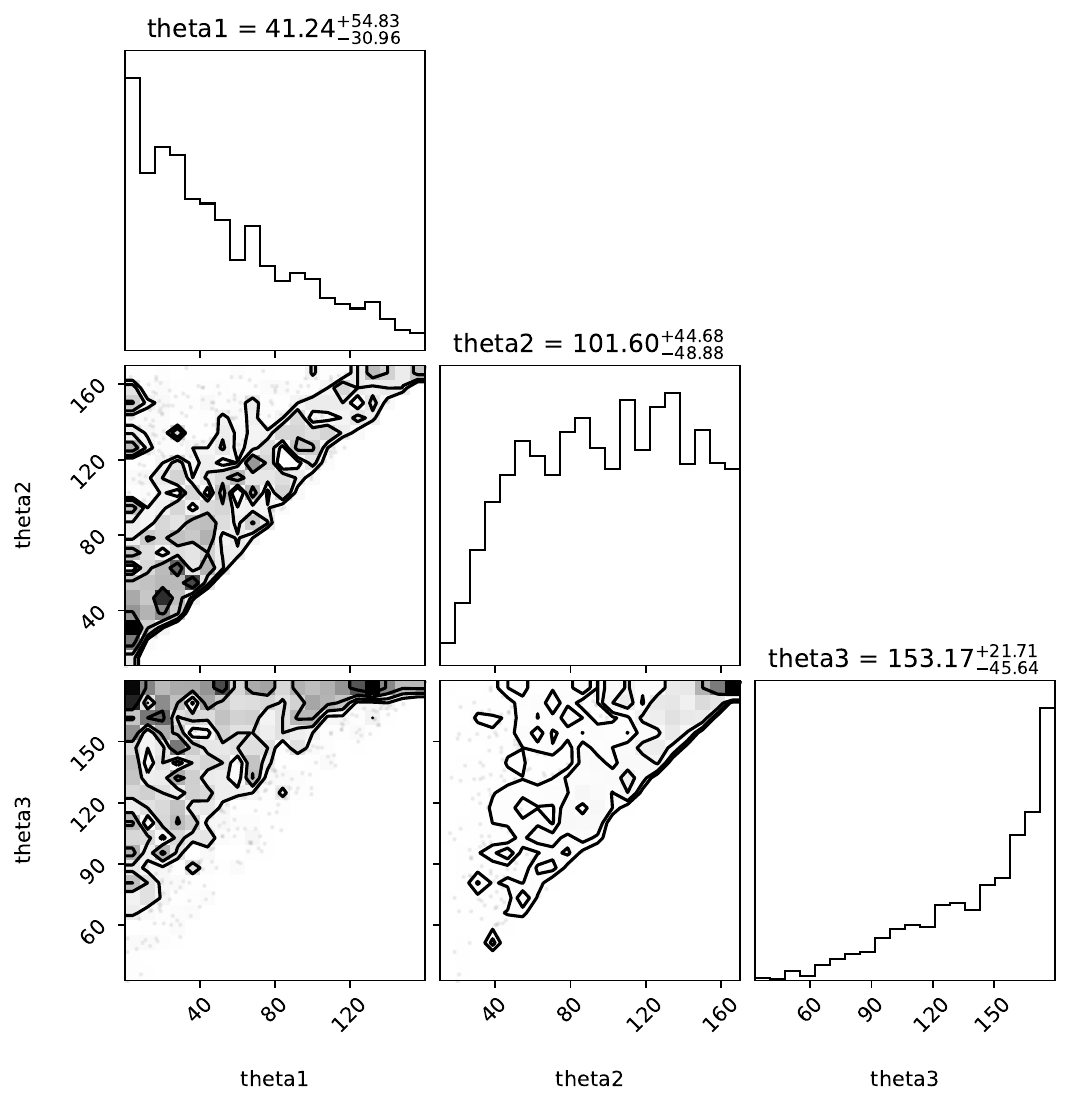
\includegraphics[width=0.5\textwidth]{corneranglesfreed-1.png}
	\caption{Corner plot mapping combinations of $\theta$ that generate the best improvement}
\end{figure}

\figurename{ 4} is the resulting corner plot from our ultranest sampler, darker areas indicate a choice of angles where the model performed better where as lighter areas are where the model did poorer. Overall from the corner plot provided it's clear that there is no direct correlation between our model's performance and the choice of detection angle. While the choice of angles does not provide a direct improvement in our estimation it does determine how finely we can estimate the orientation, for choices of angles that are close together the minimum spacing between our signals is so small that we can't achieve any greater accuracy than dividing the orientation space into 30 reference orientations. We hope to develop our model further in the future by being able to determine the maximum accuracy given that we know the signal error of our measurements.  

As covered in \ref{sec:3.2} our choice for beta can help to improve our estimation by restricting it in the physical space. By tuning our choices of $\beta$ in accordance with

\section{Conclusion}
\label{4}
We have developed a model for interpreting the dynamics of a trapped particle based purely on the light scattering pattern.

Our simulations of asymmetric dimers found that for large sphere ratios the dimer will prefer to be orientated against the beam propagation and will even move further from the trapping focus to invert itself before coming back to the laser focus. It is interesting that is only the case for dimers where the size ratio is greater than 1:2, understanding how the optical torque varies with size ratio can provide unique insight into the dynamics of non-spherical trapping targets.  

Overall the model developed can be applied to any characteristic that impacts the light scattering pattern produced by the trapped entity. The MSTM package is flexible in  calculating the light scattering for a variety of micro particles, so long as we can calculate the light scattering we can apply our model to help characterise the trapped model. We hope to extend this work for characterising continuos processes such as nucleation within an optical trap.  

The authors would like to acknowledge and thank the support for this research from the funding provided by the Leverhulme Trust.  

\bibliography{bib} 
\bibliographystyle{ieeetr}
\newpage

\section*{Appendix}
\label{Appendix 1}
\begin{table}[h]
	\begin{center}
		\caption{\label{tab:n} Reference Orientations vector components$^*$}
		\begin{tabular}{|c|c|c|c|}
			\hline\hline
			Reference Orientation & $\hat{n}_x$ &  $\hat{n}_y$ &  $\hat{n}_z$ \\
			\hline
			$1$ & $ 0.29588$ &  $ 0.29588$ & $ 0.90825$ \\
			$2$ & $ 0.90825$ &  $ 0.29588$ & $ 0.29588$ \\
			$3$ & $ 0.29588$ &  $ 0.90825$ & $ 0.29588$ \\
			$4$ & $1.0000$ &  $0.00000$ & $0.00000$ \\
			$5$ & $0.00000$ &  $1.0000$ & $0.00000$ \\
			$6$ & $0.00000$ &  $0.00000$ & $1.0000$ \\
			$7$ & $ 0.29588$ &  $ 0.29588$ & $-0.90825$ \\
			$8$ & $ 0.90825$ &  $ 0.29588$ & $-0.29588$ \\
			$9$ & $ 0.29588$ &  $ 0.90825$ & $-0.29588$ \\
			$10$ & $0.00000$ &  $0.00000$ & $-1.0000$ \\
			$11$ & $ 0.29588$ &  $-0.29588$ & $ 0.90825$ \\
			$12$ & $ 0.90825$ &  $-0.29588$ & $ 0.29588$ \\
			$13$ & $ 0.29588$ &  $-0.90825$ & $ 0.29588$ \\
			$14$ & $0.00000$ &  $-1.0000$ & $0.00000$ \\
			$15$ & $ 0.29588$ &  $-0.29588$ & $-0.90825$ \\
			$16$ & $ 0.90825$ &  $-0.29588$ & $-0.29588$ \\
			$17$ & $ 0.29588$ &  $-0.90825$ & $-0.29588$ \\
			$18$ & $-0.29588$ &  $ 0.29588$ & $ 0.90825$ \\
			$19$ & $-0.90825$ &  $ 0.29588$ & $ 0.29588$ \\
			$20$ & $-0.29588$ &  $ 0.90825$ & $ 0.29588$ \\
			$21$ & $-1.0000$ &  $0.00000$ & $0.00000$ \\
			$22$ & $-0.29588$ &  $ 0.29588$ & $-0.90825$ \\
			$23$ & $-0.90825$ &  $ 0.29588$ & $-0.29588$ \\
			$24$ & $-0.29588$ &  $ 0.90825$ & $-0.29588$ \\
			$25$ & $-0.29588$ &  $-0.29588$ & $ 0.90825$ \\
			$26$ & $-0.90825$ &  $-0.29588$ & $ 0.29588$ \\
			$27$ & $-0.29588$ &  $-0.90825$ & $ 0.29588$ \\
			$28$ & $-0.29588$ &  $-0.29588$ & $-0.90825$ \\
			$28$ & $-0.90825$ &  $-0.29588$ & $-0.29588$ \\
			$30$ & $-0.29588$ &  $-0.90825$ & $-0.29588$ \\
			\hline\hline
			\multicolumn{4}{l}{\small *Orientation vector points from centre of sphere 1 to centre of sphere 2.} \\
		\end{tabular}
	\end{center}
\end{table}


\begin{table}[h]
	\begin{center}
		\caption{\label{tab:n} Raw intensities $I_k$$^*$ and scaled intensities $y_k$}
		\begin{tabular}{|c|c|c|c|c|c|c|}
			\hline\hline
			Reference Orientation & $I_1$ &  $I_2$ &  $I_3$ & $y_1$ & $y_2$ & $y_3$ \\
			\hline
			$1$ & $13.371$ & $0.1264$ & $0.0122$ & $-0.5423$ & $-0.4253$ & $-0.4838$ \\
			$2$ & $13.237$ & $0.0272$ & $0.0102$ & $0.2429$ & $-1.401$ & $-0.7826$ \\
			$3$ & $15.840$ & $0.1072$ & $0.0234$ & $1.337$ &$-0.6142$&	$1.162$ \\
			$4$ & $12.657$ & $0.2246$ & $0.0244$ & $-0.0012$ &	$0.5399$ & $0.9695$ \\
			$5$ & $15.351$ & $0.0527$ & $0.0221$ & $1.132$ &	$-1.150$ & $1.303$ \\
			$6$ & $12.046$ & $0.0916$ & $0.0142$ & $-0.2584$ &	$-0.7676$ &	$-0.1886$ \\
			$7$ & $11.376$ & $0.0036$ & $0.0095$ & $-0.5403$ &$-1.633$ & $-0.8792$ \\
			$8$ & $13.130$ & $0.2346$ & $0.0095$ & $0.1977$ & $0.6379$ & $-0.8794$ \\
			$9$ & $15.975$ & $0.2893$ & $0.0273$ & $1.38724$ & $1.175$ & $1.726$ \\
			$10$ & $10.073$ & $0.2933$ & $0.0221$ & $-1.088$	& $1.215$ & $0.9641$ \\
			$11$ & $11.371$ & $0.1264$ & $0.0122$ & $-0.5423$ & $-0.4253$ & $-0.4838$ \\
			$12$ & $13.238$ & $0.0272$ & $0.0102$ & $0.2429$ &	$-1.401$ & $-0.7826$ \\
			$13$ & $15.840$ & $0.1072$ & $0.0234$ & $1.337$ &	$-0.6142$ & $1.162$ \\
			$14$ & $15.351$ & $0.0527$ & $0.0244$ & $1.132$ & $-1.150$ & $1.303$ \\
			$15$ & $13.376$ & $0.0036$ & $0.0095$ & $-0.5403$ & $-1.633$ & $-0.8792$ \\
			$16$ & $13.130$ & $0.2346$ & $0.0095$ & $0.1977$ & $0.6379$ & $-0.8794$ \\
			$17$ & $15.957$ & $0.2893$ & $0.0273$ & $1.387$	& $1.175$	& $1.726$ \\
			$18$ & $14.199$ & $0.0935$ & $0.0076$ & $0.6472$ & $-0.7496$ & $-1.158$ \\
			$19$ & $8.5164$ & $0.3133$ & $0.0076$ & $-1.743$ & $1.411$ & $-1.157$ \\
			$20$ & $12.961$ & $0.2420$ & $0.0188$ & $0.1267$ & $0.7113$ & $0.4765$ \\
			$21$ & $8.2160$ & $0.3217$ & $0.0142$ & $-1.869$ & $1.495$ & $-0.1890$ \\
			$22$ & $14.212$ & $0.2537$ & $0.0102$ & $0.6529$ & $0.8265$ & $-0.7835$ \\
			$23$ & $8.9280$ & $0.1398$ & $0.0123$ & $-1.570$ &	$-0.2934$ & $-0.4840$ \\
			$24$ & $13.328$ & $0.1964$ & $0.0234$ & $0.2807$ & $0.2624$ & $1.162$ \\
			$25$ & $14.199$ & $0.0935$ & $0.0076$ & $0.6472$ & $-0.7496$ & $-1.1580$ \\
			$26$ & $8.5164$ & $0.3133$ & $0.0076$ & $-1.743$	& $1.411$ & $-1.157$ \\
			$27$ & $12.961$ & $0.2420$ & $0.0188$ & $0.1267$	& $0.7113$ & $0.4765$ \\
			$28$ & $14.212$ & $0.2537$ & $0.0102$ & $0.6529$ & $0.8265$ & $-0.7835$ \\
			$29$ & $8.9280$ & $0.1398$ & $0.0122$ & $-1.570$ &	$-0.2934$ & $-0.4840$ \\
			$30$ & $13.328$ & $0.1964$ & $0.0234$ & $0.2807$ & $0.2624$ & $1.162$ \\
			\hline\hline
			\multicolumn{7}{l}{\small *$I_k$ values are calculated using MSTM package.}
		\end{tabular}
	\end{center}
\end{table}

\end{document}
\endinput
